\documentclass[12pt]{article}

% This is the preamble, load any packages you're going to use here
\usepackage{graphicx} 
\usepackage{float}
\usepackage{subcaption}
\usepackage{enumerate} % allows us to customize our lists
\setlength\parindent{0pt}
\usepackage{geometry}
    \geometry{
    left=1in,
    right=1in,
    bottom=1in
    }


\newcommand{\specialcell}[2][c]{%
  {\renewcommand{\arraystretch}{1}\begin{tabular}[#1]{@{}c@{}}#2\end{tabular}}}
  
\begin{document}

\title{\textbf{EE239AS Project 3}}
\author{Yuxin Jin \quad (104195828)\\
		Jamie Lee \quad (604589757)\\
        David Hong \quad (204588953)}
\date{\today}

\maketitle

\section*{Problem 1}
\renewcommand{\arraystretch}{1.7}%
\begin{center}
\begin{tabular}{|l | c|}
\hline
k & Total Least Squared Error \\ \hline
10 & 3644.785180 \\
50 & 69.095613 \\
100 & \textbf{6.306473} \\ \hline
\end{tabular}
\end{center}

\section*{Problem 2}
\begin{center}
\begin{tabular}{|*{11}{c|}}
\hline
kFold & 1 & 2 & 3 & 4 & 5 & 6 & 7 & 8 & 9 & 10\\ \hline
Average Absolute Error & 1.07 & 1.11 & \textbf{1.03} & 1.08 & \textbf{1.13} & 1.09 & 1.06 & 1.11 & 1.08 & 1.09 \\
\hline
\end{tabular}
\end{center}
Highest absolute error is 1.13 \\
Lowest absolute error is 1.03

\section*{Problem 3}
\begin{center}
\begin{tabular}{|*{2}{c|}}
\hline
kFold & Area Under the curve \\ \hline
1 & 5123.32 \\
2 & 5024.41 \\ 
3 & 4994.98 \\
4 & 5054.01 \\
5 & 5178.18 \\
6 & 5057.34 \\
7 & 5121.12 \\
8 & 5310.54 \\
9 & 5000.80 \\
10 & 5194.35 \\
\hline
\end{tabular}
\end{center}

\begin{figure*}[h!]
    \centering
    \begin{subfigure}[t]{0.5\textwidth}
        \centering
        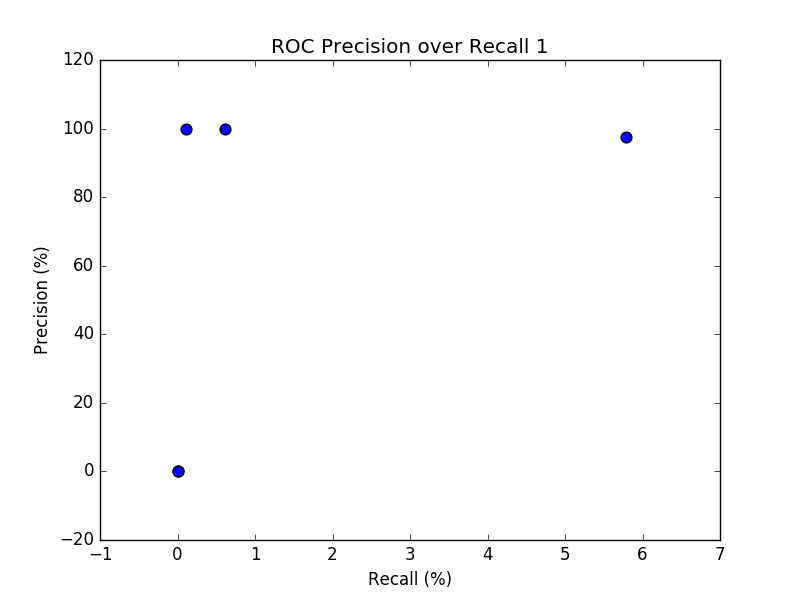
\includegraphics[width=1.\textwidth]{graphs/problem3_ROC1}
        \caption{}
    \end{subfigure}%
    ~ 
    \begin{subfigure}[t]{0.5\textwidth}
        \centering
        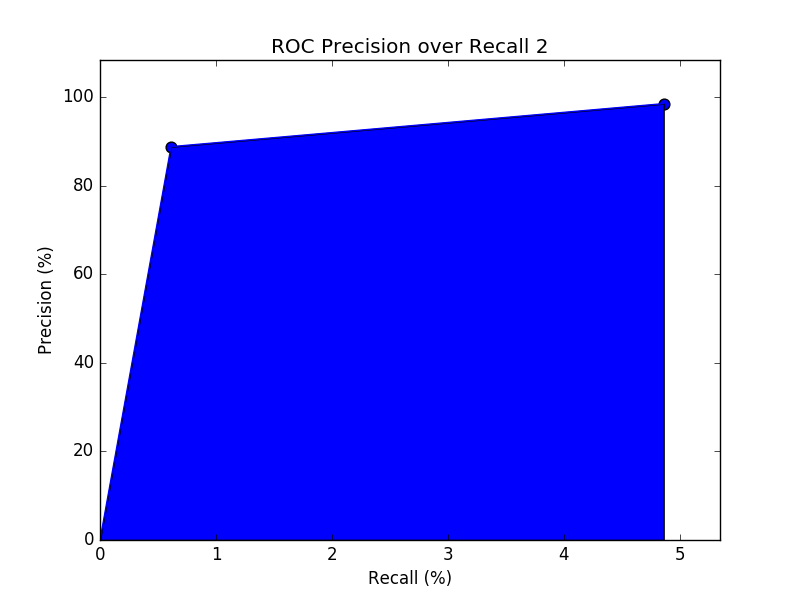
\includegraphics[width=1.\textwidth]{graphs/problem3_ROC2}
        \caption{}
    \end{subfigure}%
\end{figure*}

\begin{figure*}[h!]
\ContinuedFloat        
        \begin{subfigure}[t]{0.5\textwidth}
        \centering
        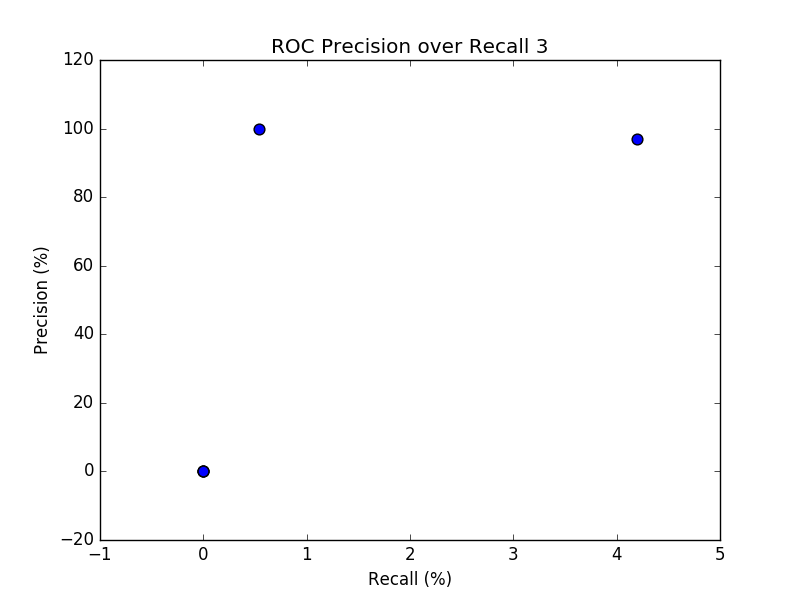
\includegraphics[width=1.\textwidth]{graphs/problem3_ROC3}
        \caption{}
    \end{subfigure}%
    ~ 
    \begin{subfigure}[t]{0.5\textwidth}
        \centering
        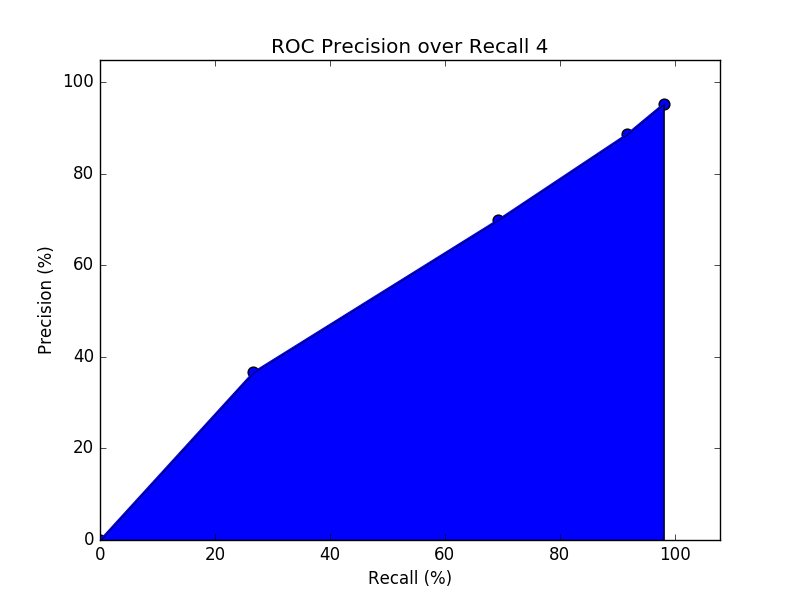
\includegraphics[width=1.\textwidth]{graphs/problem3_ROC4}
        \caption{}
    \end{subfigure}%
  
        \begin{subfigure}[t]{0.5\textwidth}
        \centering
        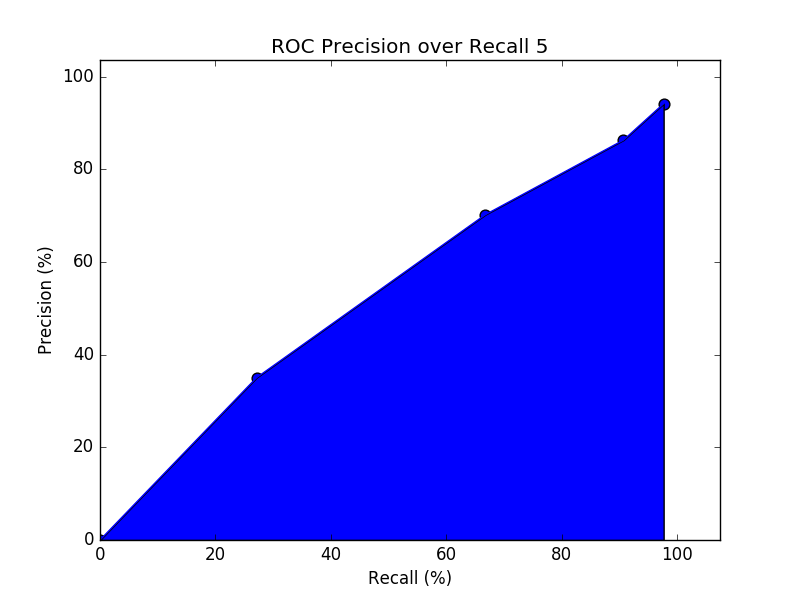
\includegraphics[width=1.\textwidth]{graphs/problem3_ROC5}
        \caption{}
    \end{subfigure}%
    ~ 
    \begin{subfigure}[t]{0.5\textwidth}
        \centering
        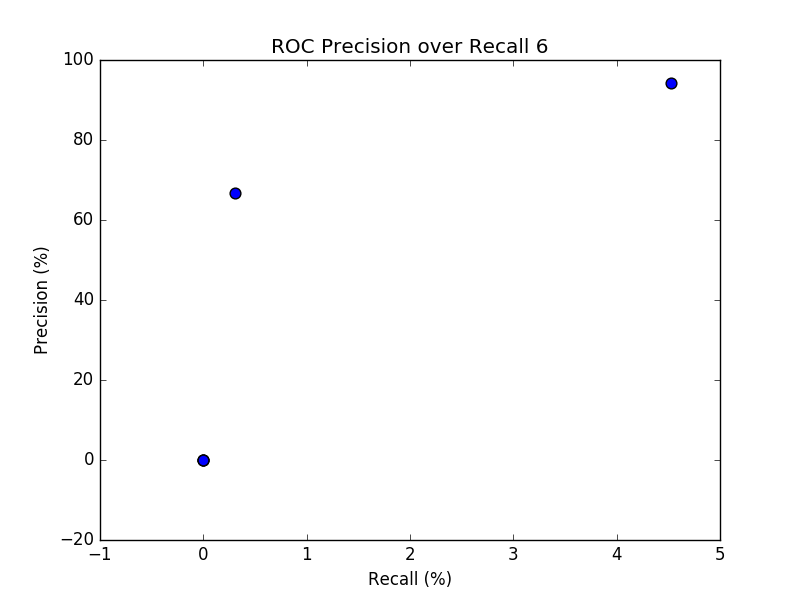
\includegraphics[width=1.\textwidth]{graphs/problem3_ROC6}
        \caption{}
    \end{subfigure}%
  
        \begin{subfigure}[t]{0.5\textwidth}
        \centering
        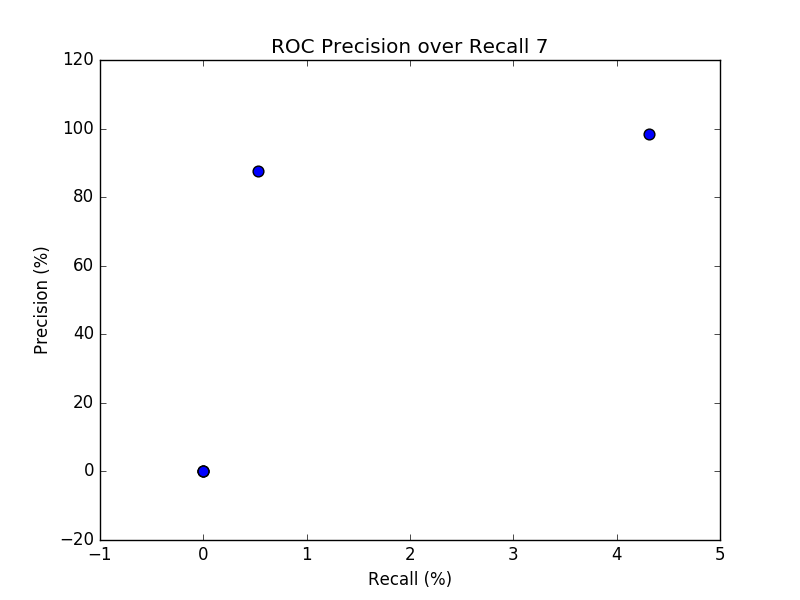
\includegraphics[width=1.\textwidth]{graphs/problem3_ROC7}
        \caption{}
    \end{subfigure}%
    ~ 
    \begin{subfigure}[t]{0.5\textwidth}
        \centering
        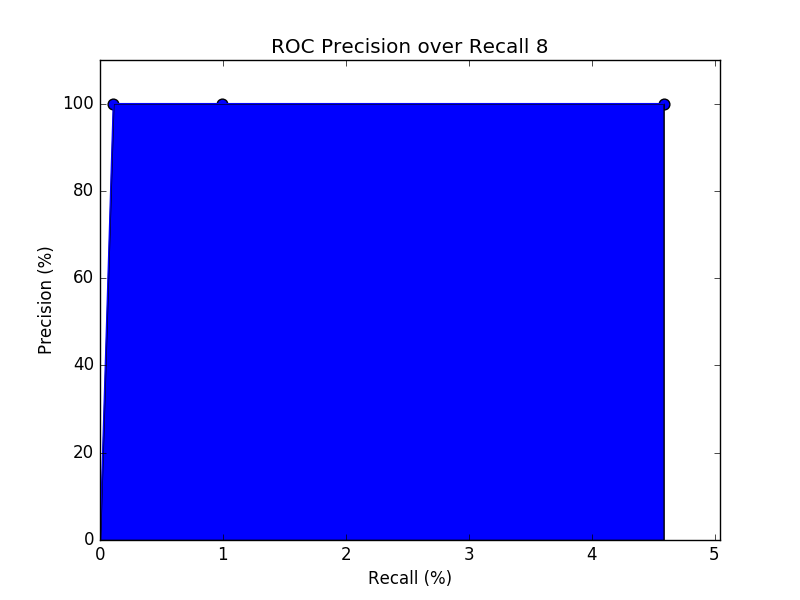
\includegraphics[width=1.\textwidth]{graphs/problem3_ROC8}
        \caption{}
    \end{subfigure}%
\end{figure*}

\begin{figure*}[h!]
\ContinuedFloat  
        \begin{subfigure}[t]{0.5\textwidth}
        \centering
        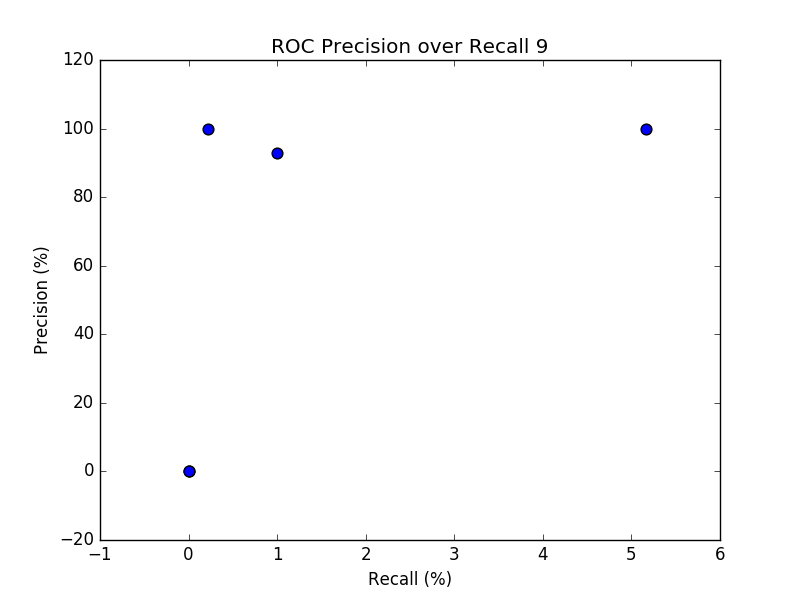
\includegraphics[width=1.\textwidth]{graphs/problem3_ROC9}
        \caption{}
    \end{subfigure}%
    ~ 
    \begin{subfigure}[t]{0.5\textwidth}
        \centering
        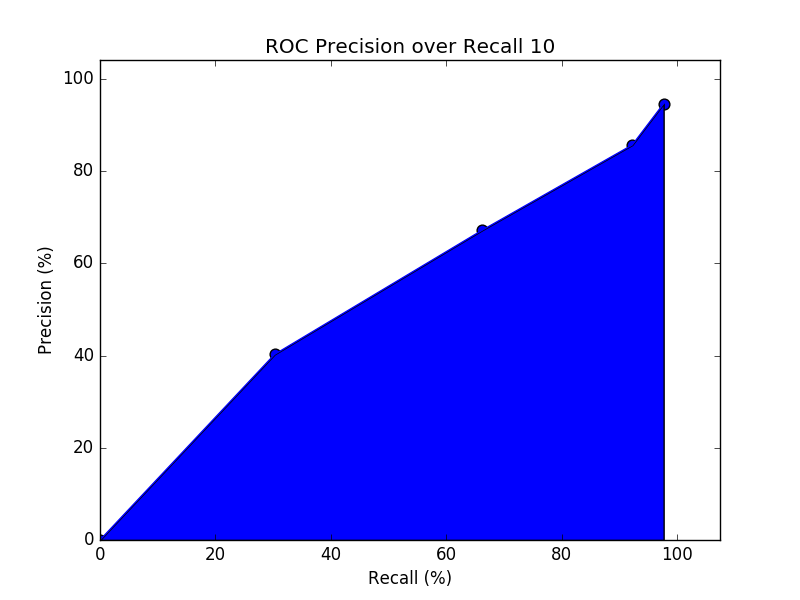
\includegraphics[width=1.\textwidth]{graphs/problem3_ROC10}
        \caption{}
    \end{subfigure}%
  
    \caption{ROC graphs of 10 cross validation sets. W have \{0, 1\} entries and R is composed of ratings.}
\end{figure*}


\section*{Problem 4}
\begin{center}
\begin{tabular}{|l | c|}
\hline
k & Total Least Squared Error \\ \hline
10 & 1.255808 \\
50 & 2.844260 \\
100 & \textbf{0.534604} \\ \hline
\end{tabular}
\end{center}

\begin{figure*}[h!]
    \centering
    \begin{subfigure}[t]{0.5\textwidth}
        \centering
        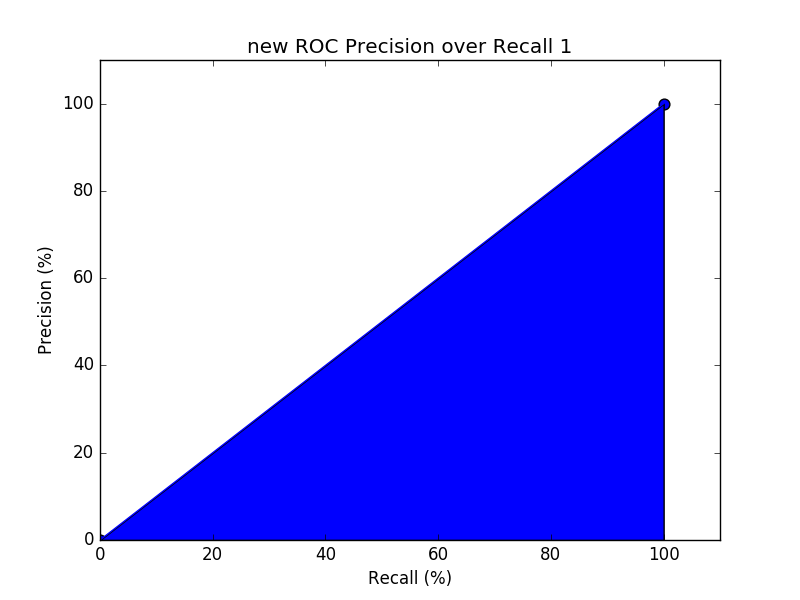
\includegraphics[width=1.\textwidth]{graphs/problem4_ROC1}
        \caption{}
    \end{subfigure}%
    ~ 
    \begin{subfigure}[t]{0.5\textwidth}
        \centering
        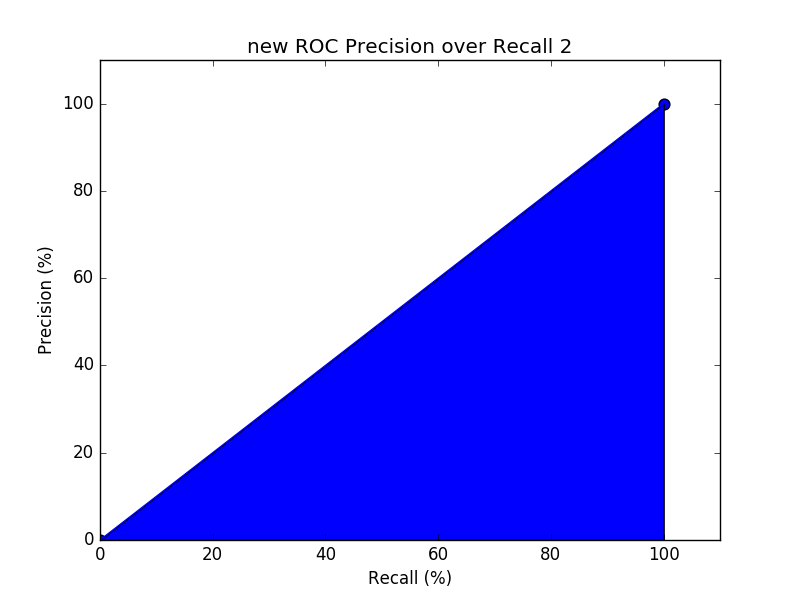
\includegraphics[width=1.\textwidth]{graphs/problem4_ROC2}
        \caption{}
    \end{subfigure}%
\end{figure*}

\begin{figure*}[h!]
\ContinuedFloat      
    \begin{subfigure}[t]{0.5\textwidth}
        \centering
        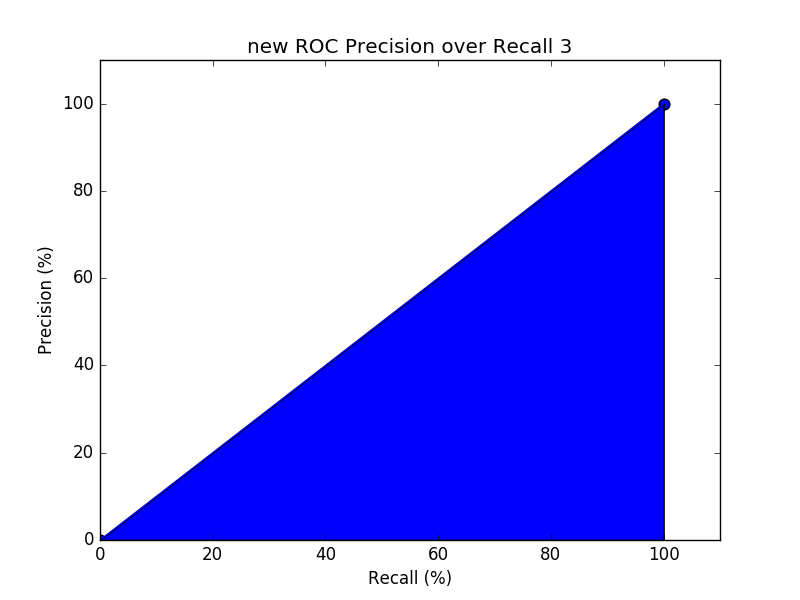
\includegraphics[width=1.\textwidth]{graphs/problem4_ROC3}
        \caption{}
    \end{subfigure}%
    ~ 
    \begin{subfigure}[t]{0.5\textwidth}
        \centering
        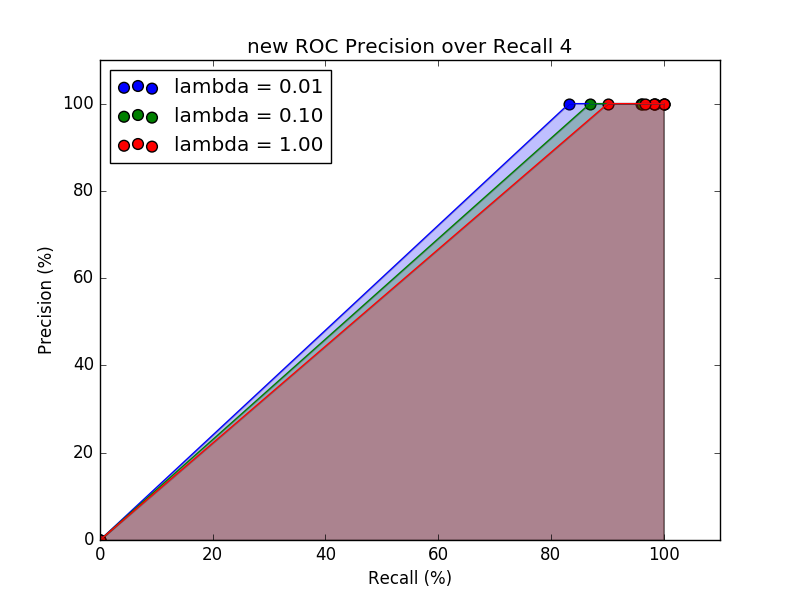
\includegraphics[width=1.\textwidth]{graphs/problem4_ROC4}
        \caption{}
    \end{subfigure}%
    
    \begin{subfigure}[t]{0.5\textwidth}
        \centering
        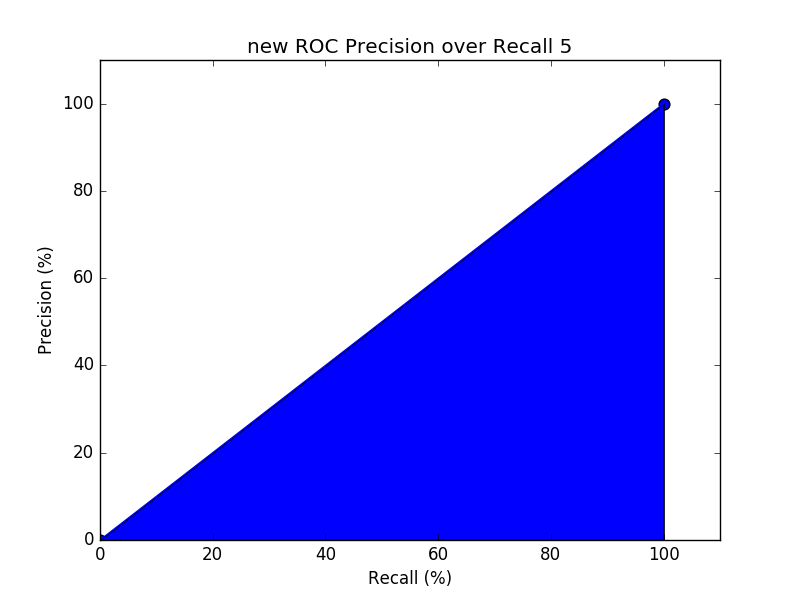
\includegraphics[width=1.\textwidth]{graphs/problem4_ROC5}
        \caption{}
    \end{subfigure}%
    ~ 
    \begin{subfigure}[t]{0.5\textwidth}
        \centering
        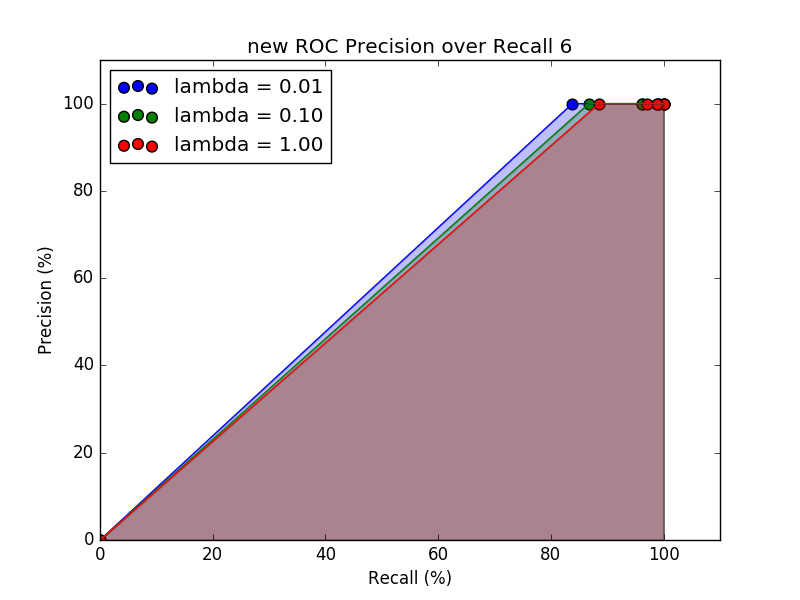
\includegraphics[width=1.\textwidth]{graphs/problem4_ROC6}
        \caption{}
    \end{subfigure}%
    
            \begin{subfigure}[t]{0.5\textwidth}
        \centering
        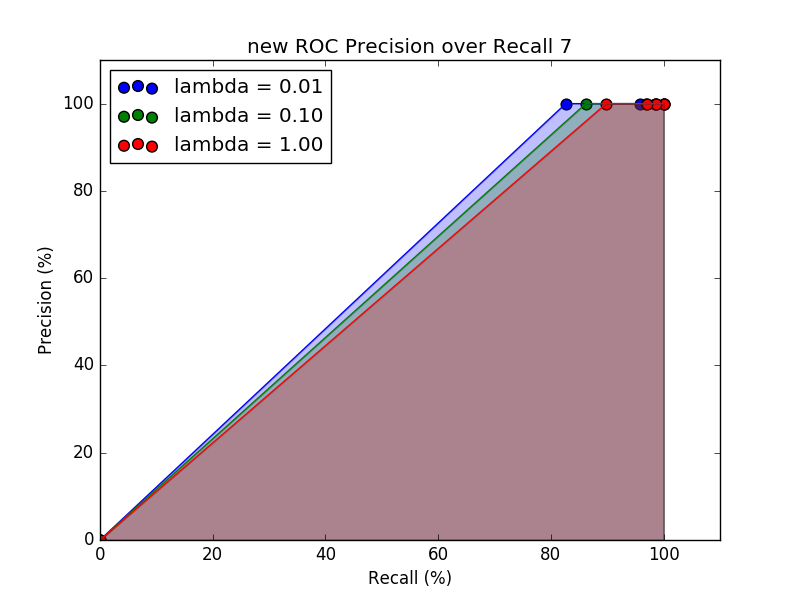
\includegraphics[width=1.\textwidth]{graphs/problem4_ROC7}
        \caption{}git 
    \end{subfigure}%
    ~ 
    \begin{subfigure}[t]{0.5\textwidth}
        \centering
        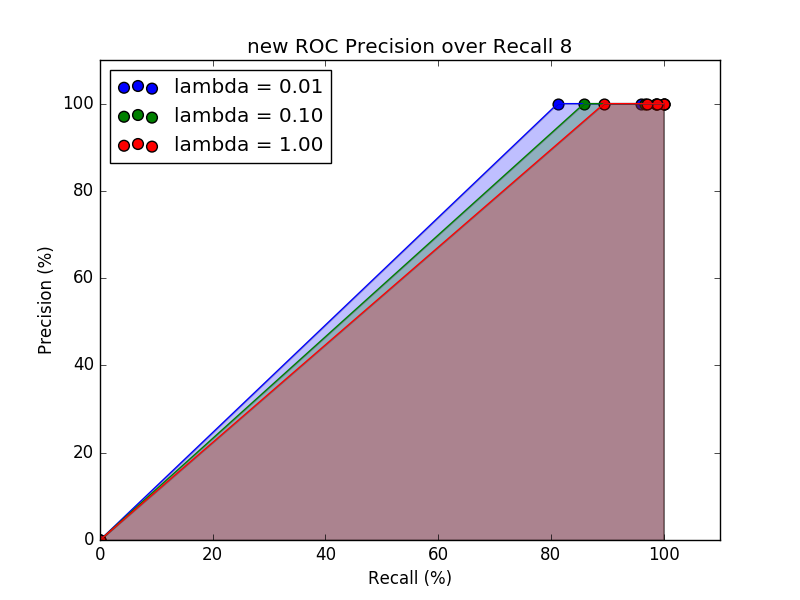
\includegraphics[width=1.\textwidth]{graphs/problem4_ROC8}
        \caption{}
    \end{subfigure}%
\end{figure*}

\begin{figure*}[h!]
\ContinuedFloat     
    \begin{subfigure}[t]{0.5\textwidth}
        \centering
        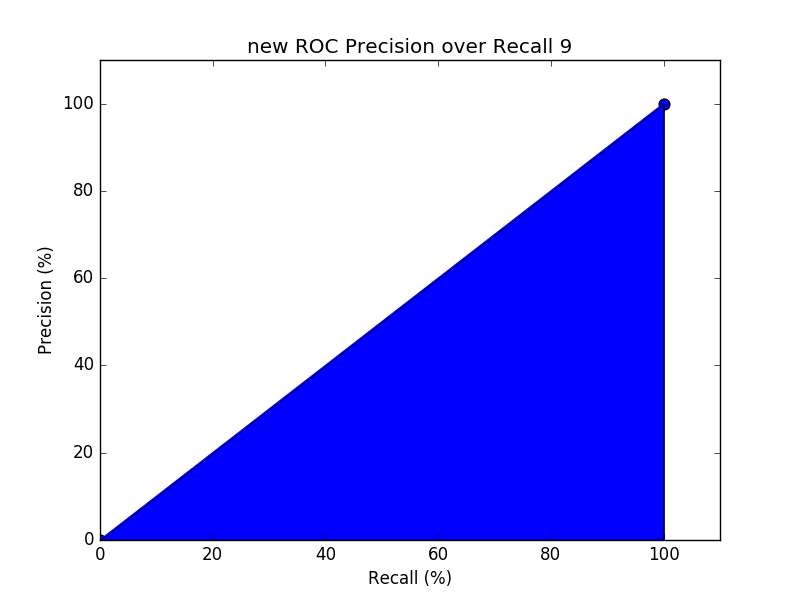
\includegraphics[width=1.\textwidth]{graphs/problem4_ROC9}
        \caption{}
    \end{subfigure}%
    ~ 
    \begin{subfigure}[t]{0.5\textwidth}
        \centering
        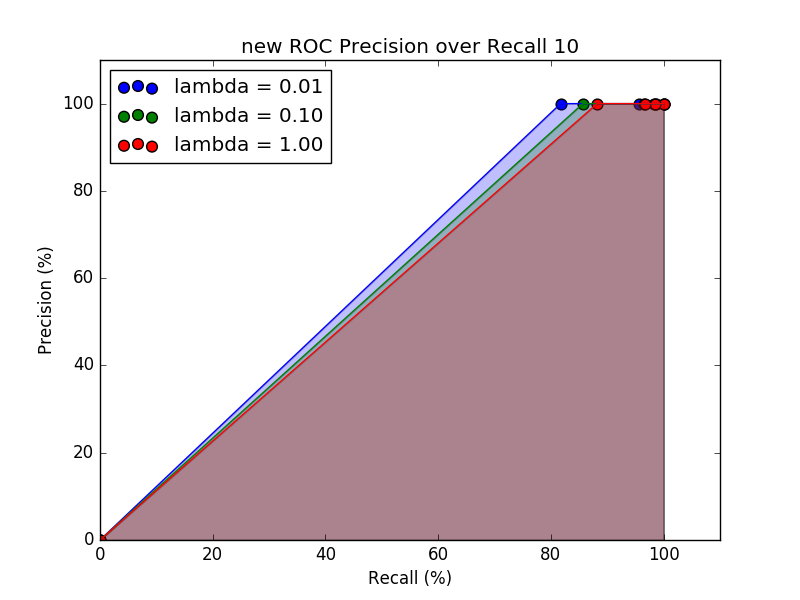
\includegraphics[width=1.\textwidth]{graphs/problem4_ROC10}
        \caption{}
    \end{subfigure}%
  
    \caption{ROC graphs of 10 cross validation sets. R have \{0, 1\} entries and weights in W are ratings.}
\end{figure*}

\section*{Problem 5}
The average precision for our collaborative filter system with $L = 5$ is $55.45\%$.
\begin{figure}[h]
\centering
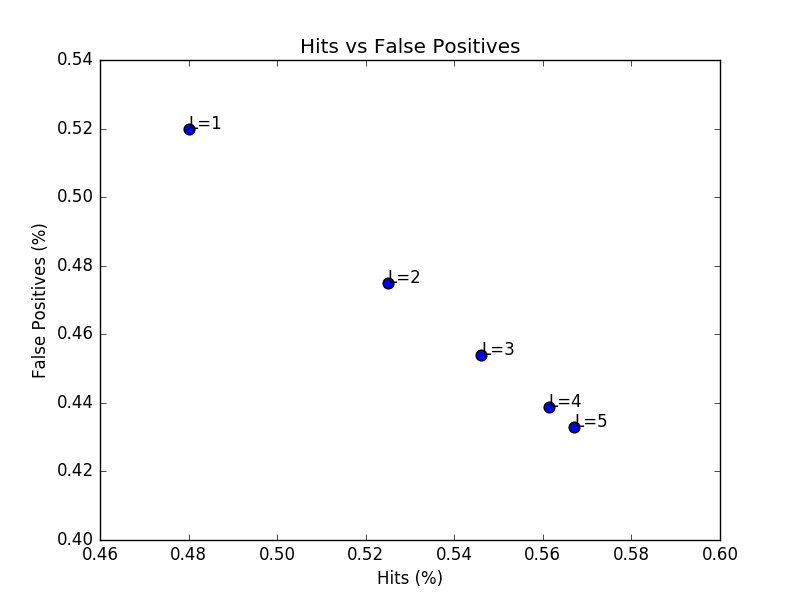
\includegraphics[width=0.55\textwidth]{graphs/problem5}
\caption{Hit vs False Positives L = 1-5}
\end{figure}

\end{document}